\section{Delineation choice: NHDPlus HR versus threshold-based DEM delineation}
\label{sec:supp-delineation}

This section provides the full controlled comparison summarized in Methods \S\ref{sec:methods-delineation}.

\subsection{Why the two networks differ in accuracy, not only in determinism}
The accuracy difference between the two delineations originates upstream of QSWAT\textsuperscript{+}, in how each network is built.
Threshold-based TauDEM extracts the channel network from the bare DEM by accumulating upslope area and cutting it at a single cell threshold, so channel-head location, channel planform, and basin divides are all functions of the terrain grid and that one cutoff \citep{Tarboton1997TauDEM, Tarboton1991ChannelNetworks}.
NHDPlus HR instead begins from the surveyed 1:24{,}000-scale NHD flowlines and the Watershed Boundary Dataset (WBD) divides and \emph{hydro-enforces} them into the 10~m 3DEP DEM---trenching (burning) the mapped streams into the surface and walling the hydrologic divides with raised cells---before deriving the elevation-based catchments and cumulative drainage area from that conditioned surface \citep{Moore2019NHDPlusHR, Moore2025NHDPlusHR}.
Consequently the channel positions, channel heads, divergences, canals, and lake and coastline boundaries reflect mapped cartography rather than an accumulation cutoff, and the catchment divides honor the official WBD boundaries---precisely the features a slope--area threshold cannot recover in flat, low-relief, karst, or leveed terrain.
Stream burning of this kind measurably improves the accuracy of DEM-derived drainage divides relative to unconditioned flow accumulation \citep{Lindsay2016StreamBurning}.
SWATGenX inherits this surveyed, hydro-enforced network when it conditions delineation on NHDPlus HR; the threshold alternative re-derives a network from the DEM and cannot reconstruct that information, which is the upstream reason the conditioned model reproduces the basin's gaged contributing area while the threshold model brackets it.

\subsection{What QSWAT\texorpdfstring{\textsuperscript{+}}{+} and the SWAT\texorpdfstring{\textsuperscript{+}}{+} Editor each require and produce}
The two delineation options enter SWATGenX at the same stage and differ only in how the stream network is defined.
QSWAT\textsuperscript{+} requires a DEM, a stream definition, and outlet/inlet points; it produces the routed channel layer (\texttt{rivs1}, carrying cumulative drainage area \texttt{AreaC}), subbasins, lake objects, and hydrologic response units.
Under NHDPlus HR conditioning the stream definition is the attributed, lake-aware national network; under the DEM-based alternative it is the set of cells whose upslope area exceeds the chosen thresholds.
The SWAT\textsuperscript{+} Editor \citep{SWATplusEditor} then consumes the QSWAT\textsuperscript{+} project database together with weather inputs and writes the executable input files (\texttt{TxtInOut}, including the routed-channel connectivity file \texttt{chandeg.con} from which contributing area at any gaged reach is read).
All quantities reported below are read from these executable artifacts rather than from intermediate GIS layers.

\subsection{A same-basin, same-DEM comparison}
We build both delineations of the small (S) benchmark domain (HUC12~\texttt{030801020804}; 52.6~km\textsuperscript{2}) as sibling projects in one model directory, on the identical 30~m DEM and the same NHD-derived lake polygons, so that the comparison isolates the delineation engine rather than the input resolution or the lake geometry (Figure~\ref{fig:taudem-delineation}).
Threshold-based TauDEM was exercised across DEM extents (a square bounding box and a basin-clipped extent), across both QSWAT\textsuperscript{+} lake-integration methods, with and without burning the NHD stream network into the DEM, and over a range of stream/channel thresholds.

\begin{figure}[htbp]
  \centering
  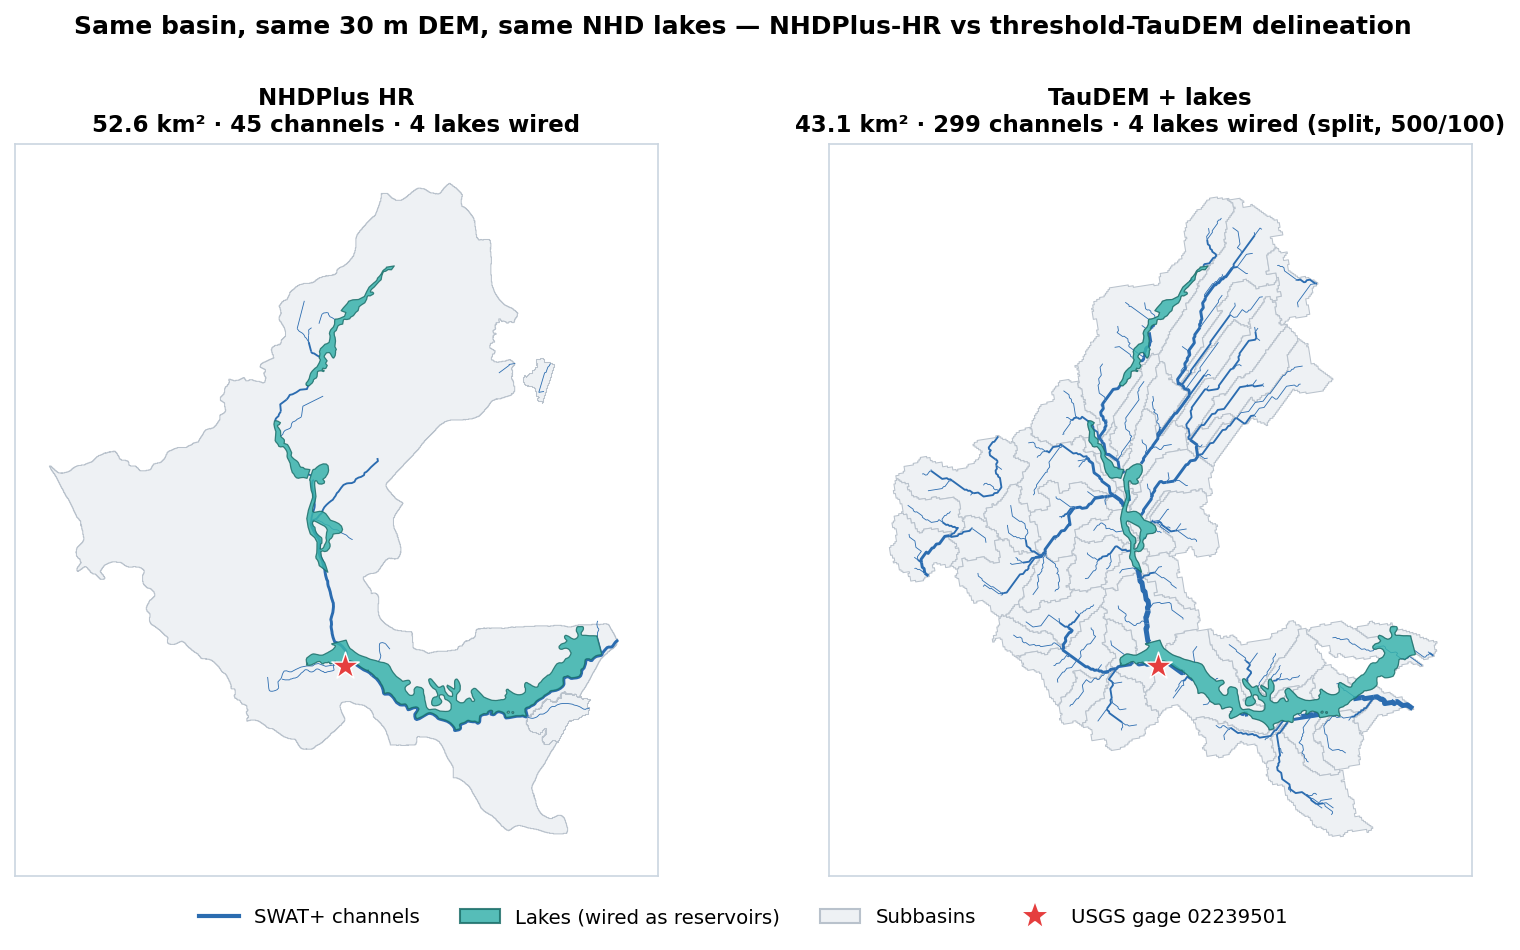
\includegraphics[width=\textwidth]{final/fig-taudem-vs-nhd-delineation-lakes.png}
  \caption{NHDPlus HR (left) and threshold-based TauDEM (right) delineations of the same 52.6~km\textsuperscript{2} benchmark basin on the identical 30~m DEM and the same NHD lake polygons. Both wire the four lakes as reservoirs; the TauDEM network is denser and more fragmented (Objective~2).}
  \label{fig:taudem-delineation}
\end{figure}

\subsection{Contributing area and lake integration}
Two differences emerge.
First, contributing area is deterministic under NHDPlus HR conditioning and extent-dependent under threshold delineation.
The NHDPlus-HR model reproduces the basin drainage area (52.6~km\textsuperscript{2}), whereas the TauDEM contributing area is set by the DEM extent: the square bounding box over-delineates (67.6~km\textsuperscript{2}) and the basin-clipped extent under-delineates (43.1~km\textsuperscript{2}), bracketing but not reproducing the conditioned value.
NHDPlus HR exposes no extent or threshold parameter, so its contributing area is fixed by the hydrography rather than chosen.
Second, the lakes can be integrated under either approach, but not equally easily.
The NHDPlus-HR model wires all four lakes as reservoir objects directly, because lake--channel topology is carried in the hydrography.
For TauDEM, the default \texttt{addHUCLakes} method fails: it resolves each lake's outlet by matching a stored NHD node identifier in the channel network, and that identifier has no counterpart in the rebuilt DEM-derived network.
The alternative \texttt{splitChannelsByLakes} method, which re-cuts channels geometrically at the lake boundaries and creates fresh outlet nodes, wires all four lakes and yields an executable model once the threshold is fine enough to thread the lake polygons (stream/channel thresholds of 500/100 cells on this basin).
Threshold-based delineation can therefore integrate the same lakes, but only with the appropriate method and a sufficiently dense network, whereas NHDPlus HR does so without per-basin tuning.

\subsection{When delineation is not the limiting factor}
A delineation comparison against observed streamflow is only meaningful where the modeled surface watershed governs the gaged flow.
The S benchmark gage (USGS~\texttt{02239501}, the Silver River) illustrates the alternative: it is fed by Silver Springs, a first-magnitude artesian spring discharging from the Upper Floridan aquifer \citep{Phelps2004SilverSprings}.
The U.S. Geological Survey reports no contributing drainage area for this site, and the observed daily flow is exceptionally stable (coefficient of variation~0.22 over 2000--2024), the hydrologic signature of groundwater discharge rather than surface runoff.
The uncalibrated simulation undersimulates the observed mean of roughly 16~m\textsuperscript{3}\,s\textsuperscript{-1} by more than an order of magnitude under \emph{both} delineations, and by an essentially identical margin, because the dominant flux originates in a regional karst aquifer that is exogenous to any surface-water delineation of the local basin (Figure~\ref{fig:taudem-hydrograph}).
Conduit-dominated karst systems are well known to be poorly represented by conceptual rainfall--runoff models without dedicated process representation \citep{Hartmann2014KarstWaterResources}, and the simplified SWAT\textsuperscript{+} groundwater store is not designed to reproduce sustained artesian spring discharge \citep{SanchezGomez2024SWATplusBaseflow}.
This is a process mismatch rather than a delineation or gage-assignment error, and it is the same for either method.
Its practical implication is that delineation cannot be judged by streamflow at gages whose hydrology the surface model does not represent; station selection must precede the comparison.

\begin{figure}[htbp]
  \centering
  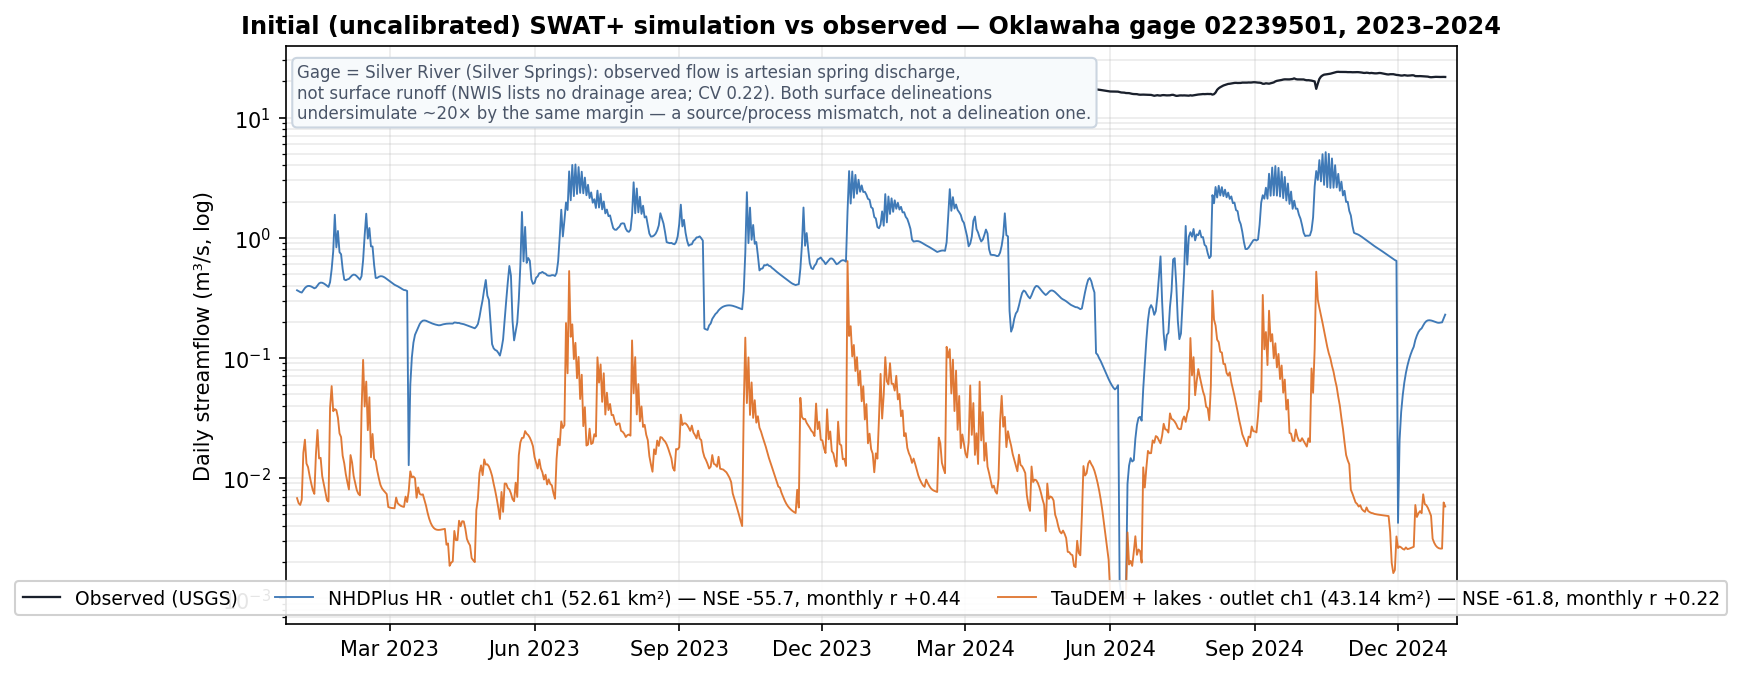
\includegraphics[width=\textwidth]{final/fig-taudem-vs-nhd-hydrograph.png}
  \caption{Initial (uncalibrated) simulated versus observed daily streamflow at USGS~\texttt{02239501} (Silver River). Both delineations undersimulate by a similar margin because the gaged flow is artesian spring discharge, exogenous to the surface-water model; the gap reflects a missing process, not the delineation (log scale; Objective~2).}
  \label{fig:taudem-hydrograph}
\end{figure}

\subsection{Station selection and the watershed-scale comparison}
We scale the comparison to the Peace River HUC8 (\texttt{03100101}; 6{,}030~km\textsuperscript{2}, 63 HUC12 subwatersheds, 76 USGS gages) under an explicit station-selection rule that follows from the preceding observation.
Gages are retained only when their assignment class is calibration-ready (\S\ref{sec:methods-drainage-audit}: tributary or mainstem reaches with at most a documented area offset) and when their observed record represents surface runoff: gages on lakes and canals, tidal or bidirectional reaches, gages with insufficient record coverage, and spring-dominated runs (identified by an anomalously low flow coefficient of variation) are excluded.
On Peace this retains 21 runoff-dominated gages from the 76-gage inventory.

At this scale the two approaches diverge not only in how many gages remain usable for calibration but in what it takes to obtain an executable model at all.
The NHDPlus-HR--conditioned delineation builds the Peace basin cleanly and runs in a single unattended pass---on the order of one to two hours of wall-clock---inheriting its 347 mapped waterbodies as lake objects directly from the hydrography, with no per-basin intervention.
Threshold-based TauDEM does not preclude a lake-bearing Peace model, but reaching one is a per-basin search over the stream and channel thresholds and the DEM resolution rather than a single run, and in that search each delineation attempt is itself a multi-hour build; the configuration we converged on produced a runnable model only by omitting the lakes.
Two configurations did not complete in our trials: a fine network (stream/channel thresholds of 1250--5000 / 250--1000 cells) with lake integration ran its lake-topology merge over hundreds of subbasins and 347 waterbodies for more than eight hours without producing hydrologic response units; and a coarse network (stream threshold $\approx$~30{,}000--106{,}000 cells) with lakes terminated abnormally during lake integration.
A coarse network with the lakes omitted also stalled during HRU construction until the DEM was additionally clipped to the basin polygon and only the surveyed StreamRiver flowlines were burned into it.
With that full combination---coarse auto-threshold, basin-clipped DEM, a flowline-type-selective burn of the major rivers, and the 347 lakes dropped---QSWAT\textsuperscript{+} did complete, yielding the first runnable threshold-delineated Peace SWAT\textsuperscript{+} model we obtained.
That model is not a parity result. It carries none of the basin's 347 waterbodies---though, as on the small basin, lakes can be wired back with a denser network and the geometric \texttt{splitChannelsByLakes} method at further tuning cost; it is heavily over-segmented relative to the conditioned network (2{,}304 subbasins and 22{,}361 channels, against 162 subbasins and 8{,}181 channels for NHDPlus HR); and its total contributing area agrees with the hydrography (5{,}853 versus 5{,}982~km\textsuperscript{2}, within 2\%) only because the DEM was clipped to the basin polygon, suppressing the cross-divide over-capture an unclipped threshold delineation otherwise produces.
Crucially, even where the contributing area matches, the internal network the threshold method lays down is a flow-accumulation reconstruction---an arbitrary routing of the surface water---rather than the surveyed path: the same conditioned-network properties that make NHDPlus HR deterministic on the small basin (a surveyed, lake-aware topology supplied to QSWAT\textsuperscript{+} rather than reconstructed from the DEM) are what let it build a large, lake-dense basin unattended and with its waterbodies and routing intact.

For the 21 retained gages we therefore evaluate the NHDPlus-HR model's uncalibrated initial simulation against observed daily flow, cross-validating the gage-to-channel assignment across the full channel set rather than relying on a single nearest-channel pick.
The watershed-scale point is therefore not that a threshold delineation is impossible but that obtaining one is a costly per-basin search whose product is an arbitrary surface-water routing: tolerable where a model is calibrated to a single gage whose contributing area matches, yet consequential where delineation accuracy drives local-scale water-resource decisions and their policy implementation, since those decisions turn on where water actually routes and which channel carries it. Conditioning on a surveyed hydrography removes that routing uncertainty by construction and is what makes an unattended, lake-faithful build of a large, lake-dense basin feasible in a single deterministic pass.
Network density---and, at the limit, buildability---rather than timing agreement alone, governs how much of a gage inventory an automated delineation can ultimately serve.

\subsection{Rationale}
The evidence favors NHDPlus-HR conditioning on two grounds rather than a claim that threshold delineation is incapable.
The first is determinism: the conditioned contributing area is fixed by the hydrography, whereas the threshold-based area depends on an extent and threshold choice that the analyst must make and defend.
The second is correctness without per-basin tuning: lakes are wired and gages carry usable cumulative drainage area directly, whereas the DEM-based alternative required a specific lake method and threshold to integrate the same lakes on the small basin, and on the large lake-dense basin could only be made to build by clipping the DEM, selectively burning the major rivers, and removing the lakes altogether.
For an automated generator intended to run unattended across thousands of domains, these properties---rather than a difference in attainable accuracy on any single basin---are the operative advantage.
